\documentclass[a4paper,12pt]{beamer}
% -------------------------------------------------
% Theme
% -------------------------------------------------
\usetheme{Berkeley}
% -------------------------------------------------
% Packages
% -------------------------------------------------
\usepackage{tabularx}
\usepackage{array}
\usepackage{graphicx}
\usepackage{listings}
\usepackage{hyperref}
\usepackage{color}
\usepackage{tikz}
\usepackage{pgfplots}
\usepackage[T1]{fontenc}
\usepackage[utf8]{inputenc}
\pgfplotsset{compat=1.18}
\usetikzlibrary{arrows.meta,positioning,shapes.geometric,matrix}
% -------------------------------------------------
% Colors
% -------------------------------------------------
\definecolor{lightgray}{gray}{0.95}
% -------------------------------------------------
% Table of contents styling
% -------------------------------------------------
\setbeamerfont{section in toc}{size=\small}
\setbeamerfont{subsection in toc}{size=\scriptsize}
% -------------------------------------------------
% Listings configuration
% -------------------------------------------------
\lstset{
    language=SQL,
    showspaces=false,
    numbers=left,
    numberstyle=\tiny,
    backgroundcolor=\color{lightgray},
    keywordstyle=\color{blue}\bfseries,
    commentstyle=\color{gray},
    stringstyle=\color{orange},
    basicstyle=\ttfamily\scriptsize,
    breaklines=true,
    literate=
        {é}{{\'e}}1
        {è}{{\`e}}1
        {à}{{\`a}}1
        {ù}{{\`u}}1
        {ç}{{\c{c}}}1
        {ô}{{\^o}}1
        {ê}{{\^e}}1
}
% -------------------------------------------------
% Presentation information
% -------------------------------------------------
\title{Comment minimiser le temps d'exécution de requêtes SQL itérées ?}
\author[Eliott P. \& Antoine BP]{Antoine Bertin--Paillette}
\date{2026}
% -------------------------------------------------
% Footer
% -------------------------------------------------
\setbeamertemplate{footline}{
    \begin{beamercolorbox}[
        wd=\paperwidth,
        ht=2.5ex,
        dp=1ex
    ]{author in head/foot}
        \usebeamerfont{author in head/foot}
        \hspace*{2ex}
        \insertshortauthor
        \hfill
        \inserttitle
        \hfill
        \insertdate
        \hfill
        \insertframenumber/\inserttotalframenumber
        \hspace*{2ex}
    \end{beamercolorbox}
}
\setbeamertemplate{navigation symbols}{}
% -------------------------------------------------
% Compact top header
% -------------------------------------------------
\setbeamertemplate{headline}{
    \leavevmode
    \begin{beamercolorbox}[
        wd=\paperwidth,
        ht=1.5ex,
        dp=0.6ex
    ]{section in head/foot}
    \end{beamercolorbox}
}
% -------------------------------------------------
% Sidebar configuration
% -------------------------------------------------
\setbeamersize{sidebar width left=2.4cm}
\setbeamertemplate{sidebar left}{
    \vspace{0.5em}
    \insertverticalnavigation{\beamersidebarwidth}
}
\setbeamerfont{section in sidebar}{size=\scriptsize}
\setbeamerfont{subsection in sidebar}{size=\tiny}
\setbeamercolor{section in sidebar}{fg=white, bg=blue!75}
\setbeamercolor{section in sidebar shaded}{fg=white!75}
\setbeamercolor{subsection in sidebar}{fg=white!90, bg=blue!25}
\setbeamercolor{subsection in sidebar shaded}{fg=white!65}

% -------------------------------------------------
\begin{document}

\begin{frame}
    \titlepage
\end{frame}

\begin{frame}
    \frametitle{Sommaire}
    \tableofcontents[hideallsubsections]
\end{frame}

% =================================================
\section{But du TIPE}
% =================================================

\subsection{Description du jeu de données}

\begin{frame}{Description du jeu de données}
    \begin{block}{Nous avons choisi de travailler sur les données de Wikipédia}
        \begin{itemize}
            \item Des données de \textbf{pages} : titre, contenu, thème, modifications
            \item Des données d'\textbf{utilisateurs} : nom, date d'inscription, nombre de modifications
            \item Des \textbf{révisions} de pages
        \end{itemize}
    \end{block}
    \vspace{0.3cm}
    \begin{columns}[T]
        \column{0.48\textwidth}
        \scriptsize
        \centering
        \textbf{Table \texttt{pages} (extrait)}\\[4pt]
        \begin{tabular}{r c l}
            \textbf{id} & \textbf{ns} & \textbf{title} \\
            \hline
            3  & 0 & Antoine Meillet \\
            10 & 0 & Algorithmique \\
            15 & 0 & Autriche \\
            18 & 0 & Arsène Lupin \\
            27 & 0 & Ada (langage) \\
        \end{tabular}

        \column{0.48\textwidth}
        \scriptsize
        \centering
        \textbf{Table \texttt{revisions} (extrait)}\\[4pt]
        \begin{tabular}{r r r}
            \textbf{id} & \textbf{parent\_id} & \textbf{contrib.} \\
            \hline
            230038204 & 226458976 & 316223 \\
            226672222 & 216521656 & 5256901 \\
            228034381 & 228034155 & 1430140 \\
        \end{tabular}
    \end{columns}
\end{frame}

\subsection{Que faire des résultats ?}

\begin{frame}{Que faire des résultats ?}
    \begin{columns}[T]
        \column{0.48\textwidth}
        \begin{block}{Requêtes typiques}
            \begin{itemize}
                \item Classement des utilisateurs les plus actifs par catégorie
                \item Utilisateurs experts d'une catégorie
                \item Pages les plus modifiées par catégorie
            \end{itemize}
        \end{block}

        \column{0.48\textwidth}
        \begin{block}{Utilisations des résultats}
            \begin{itemize}
                \item Récolter et afficher des statistiques utilisateur
                \item Trier, comparer, sélectionner
                \item Recommander / rechercher des pages selon des critères
            \end{itemize}
        \end{block}
    \end{columns}
\end{frame}

\begin{frame}[fragile]{Exemples de requêtes SQL}
\scriptsize
\begin{block}{1. Classement des utilisateurs les plus actifs par catégorie}
\begin{lstlisting}
SELECT c.category_name, u.username, COUNT(*) AS edits
FROM revisions r
JOIN users      AS u ON r.user_id    = u.user_id
JOIN pages      AS p ON r.page_id    = p.page_id
JOIN categories AS c ON p.category_id = c.category_id
GROUP BY c.category_name, u.username
ORDER BY c.category_name, edits DESC;
\end{lstlisting}
\end{block}
\vspace{-0.15cm}
\begin{block}{2. Pages les plus modifiées par catégorie}
\begin{lstlisting}
SELECT c.category_name, p.title, COUNT(*) AS revisions
FROM revisions r
JOIN pages      AS p ON r.page_id    = p.page_id
JOIN categories AS c ON p.category_id = c.category_id
GROUP BY c.category_name, p.title
ORDER BY revisions DESC;
\end{lstlisting}
\end{block}
\end{frame}

% =================================================
\section{Réalisation}
% =================================================

\subsection{Ce qui est prévu}

\begin{frame}{Ce qui est prévu}
    \begin{block}{Objectif : comparer nos performances aux solutions existantes}
        \centering
        \vspace{0.1cm}
        \begin{tikzpicture}
        \begin{axis}[
            width=0.88\textwidth,
            height=0.42\textheight,
            ybar,
            bar width=7pt,
            ymin=0, ymax=115,
            ylabel={\scriptsize Temps relatif (base ligne = 100)},
            symbolic x coords={Lecture, Agrégation, GROUP BY, Jointure},
            xtick=data,
            xticklabel style={font=\scriptsize},
            legend style={at={(0.5,1.02)}, anchor=south,
                          legend columns=3, font=\scriptsize},
            nodes near coords,
            nodes near coords style={font=\tiny},
            enlarge x limits=0.2,
            grid=major
        ]
        \addplot+[draw=gray,fill=gray!40] coordinates {
            (Lecture,100)(Agrégation,100)(GROUP BY,100)(Jointure,100)};
        \addplot+[draw=blue!70,fill=blue!30] coordinates {
            (Lecture,6)(Agrégation,12)(GROUP BY,10)(Jointure,15)};
        \addplot+[draw=orange!80,fill=orange!40,dashed] coordinates {
            (Lecture,0)(Agrégation,0)(GROUP BY,0)(Jointure,0)};
        \legend{Base lignes, Base colonnes, Nos performances (à mesurer)}
        \end{axis}
        \end{tikzpicture}
        \vspace{0.1cm}
    \end{block}
    {\tiny Les barres « Nos performances » seront remplies après mesures expérimentales.}
\end{frame}

\subsection{Ce qui a été fait}

\begin{frame}{Ce qui a été fait}
    \begin{columns}[T]
        \column{0.48\textwidth}
        \begin{block}{Implémenté}
            \begin{itemize}
                \item BDD fonctionnelle pour la plupart des requêtes
                \item Optimisations du plan d'exécution
                \item Optimisations mémoire
            \end{itemize}
        \end{block}

        \column{0.48\textwidth}
        \begin{block}{En cours / À faire}
            \begin{itemize}
                \item Tests sur un grand nombre de requêtes et enregistrement des temps
                \item Comparaison avec des implémentations existantes
                \item Amélioration des parties imparfaites
            \end{itemize}
        \end{block}
    \end{columns}
\end{frame}

% =================================================
\section{Optimisations mémoire}
% =================================================

\subsection{Paradigme ligne VS colonne}

\begin{frame}{Paradigme ligne VS colonne}
    \begin{columns}[T]
        \column{0.48\textwidth}
        \begin{block}{Orientée lignes}
            \footnotesize
            \begin{itemize}
                \item Stockage par enregistrement complet
                \item Efficace pour \texttt{SELECT *} et OLTP
                \item Lit des colonnes inutiles pour les agrégations
            \end{itemize}
        \end{block}
        \vspace{0.2cm}
        \begin{exampleblock}{Exemple (PostgreSQL, MySQL)}
            \centering\scriptsize
            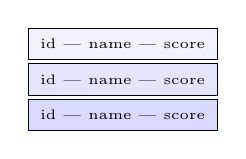
\begin{tikzpicture}
                \draw[fill=blue!15] (0,0) rectangle (2.4,0.4)
                    node[midway]{\tiny id | name | score};
                \draw[fill=blue!10] (0,0.45) rectangle (2.4,0.85)
                    node[midway]{\tiny id | name | score};
                \draw[fill=blue!5]  (0,0.9)  rectangle (2.4,1.3)
                    node[midway]{\tiny id | name | score};
            \end{tikzpicture}
        \end{exampleblock}

        \column{0.48\textwidth}
        \begin{block}{Orientée colonnes}
            \footnotesize
            \begin{itemize}
                \item Stockage par attribut
                \item Meilleure compression
                \item Très efficace pour les agrégations analytiques
            \end{itemize}
        \end{block}
        \vspace{0.2cm}
        \begin{exampleblock}{Exemple (DuckDB, C-Store)}
            \centering\scriptsize
            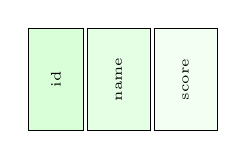
\begin{tikzpicture}
                \draw[fill=green!15] (0,0)    rectangle (0.7,1.3)
                    node[midway,rotate=90]{\tiny id};
                \draw[fill=green!10] (0.75,0) rectangle (1.55,1.3)
                    node[midway,rotate=90]{\tiny name};
                \draw[fill=green!5]  (1.6,0)  rectangle (2.4,1.3)
                    node[midway,rotate=90]{\tiny score};
            \end{tikzpicture}
        \end{exampleblock}
    \end{columns}
    \vfill
    {\tiny Source : Abadi et al., \textit{Column-Stores vs. Row-Stores} (SIGMOD 2008)}
\end{frame}

\begin{frame}{Bases orientées colonnes vs orientées lignes}
\small
\begin{block}{Temps d'exécution normalisés (base ligne = 100)}
\centering\tiny Requêtes analytiques typiques : \texttt{SUM}, \texttt{GROUP BY}, jointures.
\end{block}
\vspace{-0.15cm}
\begin{center}
\begin{tikzpicture}
\begin{axis}[
    width=0.92\textwidth,
    height=0.44\textheight,
    ybar,
    bar width=7pt,
    ymin=0, ymax=115,
    ylabel={Temps relatif (base ligne = 100)},
    symbolic x coords={
        Lecture\\3 colonnes,
        Agrégation\\SUM,
        GROUP BY,
        Jointure\\analytique
    },
    xtick=data,
    xticklabel style={align=center, font=\scriptsize},
    legend style={at={(0.5,1.02)}, anchor=south,
                  legend columns=3, font=\scriptsize},
    nodes near coords,
    nodes near coords style={font=\tiny},
    enlarge x limits=0.2,
    grid=major
]
\addplot coordinates {
    (Lecture\\3 colonnes,100)(Agrégation\\SUM,100)
    (GROUP BY,100)(Jointure\\analytique,100)};
\addplot coordinates {
    (Lecture\\3 colonnes,6)(Agrégation\\SUM,12)
    (GROUP BY,10)(Jointure\\analytique,15)};
\addplot coordinates {
    (Lecture\\3 colonnes,18)(Agrégation\\SUM,25)
    (GROUP BY,20)(Jointure\\analytique,30)};
\legend{Base orientée lignes, Base orientée colonnes, Nos performances}
\end{axis}
\end{tikzpicture}
\end{center}
\vspace{-0.15cm}
{\tiny
Sources : Abadi et al., \textit{Column-Stores vs. Row-Stores} (SIGMOD 2008) ;
\textit{The Design and Implementation of Modern Column-Oriented Database Systems} (2013).
}
\end{frame}

\subsection{Indexation des données}

\begin{frame}{Indexation des données}
    \begin{columns}[T]
        \column{0.44\textwidth}
        \begin{block}{Principe}
            \footnotesize
            \begin{itemize}
                \item Structure auxiliaire pointant vers les données
                \item Évite le parcours séquentiel complet
                \item Compromis : vitesse de lecture vs coût d'écriture
            \end{itemize}
        \end{block}
        \vspace{0.2cm}
        \begin{alertblock}{Sans index}
            \centering\scriptsize
            Parcours complet de la table\\
            $\Rightarrow$ $\mathcal{O}(n)$ lectures
        \end{alertblock}
        \vspace{0.15cm}
        \begin{exampleblock}{Avec index B+}
            \centering\scriptsize
            Navigation arborescente\\
            $\Rightarrow$ $\mathcal{O}(\log n)$ lectures
        \end{exampleblock}

        \column{0.53\textwidth}
        \centering
        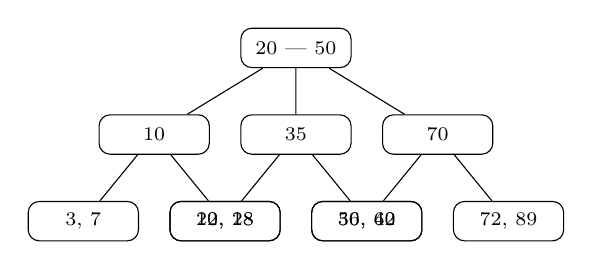
\begin{tikzpicture}[
            level distance=1.1cm,
            sibling distance=1.8cm,
            every node/.style={
                draw, rounded corners,
                minimum width=1.4cm, minimum height=0.5cm,
                font=\scriptsize
            }
        ]
        \node {20 | 50}
            child { node {10}
                child { node {3, 7} }
                child { node {12, 18} }
            }
            child { node {35}
                child { node {20, 28} }
                child { node {36, 42} }
            }
            child { node {70}
                child { node {50, 60} }
                child { node {72, 89} }
            };
        \end{tikzpicture}
        \vspace{0.15cm}
        {\scriptsize Exemple simplifié d'un arbre B+.}
    \end{columns}
    \vfill
    {\tiny Sources : Ramakrishnan \& Gehrke, \textit{Database Management Systems} ;
    Silberschatz et al., \textit{Database System Concepts}.}
\end{frame}

\begin{frame}{Index B+ : bénéfices et compromis}
\small
\begin{block}{}
\end{block}
\vspace{-0.15cm}
\begin{center}
\begin{tikzpicture}
\begin{axis}[
    width=0.92\textwidth,
    height=0.44\textheight,
    ybar,
    bar width=9pt,
    ymin=0, ymax=135,
    ylabel={Coût relatif (sans index = 100)},
    symbolic x coords={Recherche, Requête\\filtrée, Insertion, Mémoire},
    xtick=data,
    xticklabel style={align=center, font=\scriptsize},
    legend style={at={(0.5,1.02)}, anchor=south,
                  legend columns=2, font=\scriptsize},
    nodes near coords,
    nodes near coords style={font=\tiny},
    enlarge x limits=0.15,
    grid=major
]
\addplot coordinates {
    (Recherche,100)(Requête\\filtrée,100)
    (Insertion,100)(Mémoire,50)};
\addplot coordinates {
    (Recherche,8)(Requête\\filtrée,12)
    (Insertion,120)(Mémoire,115)};
\legend{Sans index, Index B+}
\end{axis}
\end{tikzpicture}
\end{center}
\vspace{-0.1cm}
\begin{alertblock}{Observation}
\small
Un index B+ réduit fortement le coût des recherches ($\mathcal{O}(\log n)$),
mais ralentit les insertions car l'arbre doit rester équilibré.
\end{alertblock}
{\tiny Valeurs normalisées (sans index = 100). Sources : Silberschatz et al. ; Ramakrishnan \& Gehrke.}
\end{frame}

\subsection{Fragmentation des données}

\begin{frame}{Fragmentation des données (Database Cracking)}
    \begin{columns}[T]
        \column{0.48\textwidth}
        \begin{block}{Principe}
            \footnotesize
            \begin{itemize}
                \item Réorganisation \textbf{à la volée} lors des requêtes
                \item Pas d'index préconstruit : l'index se forme progressivement
                \item Chaque requête améliore la structure pour les suivantes
            \end{itemize}
        \end{block}
        \vspace{0.2cm}
        \begin{exampleblock}{Avantages}
            \footnotesize
            \begin{itemize}
                \item Pas de surcoût d'initialisation
                \item S'adapte aux requêtes réelles
            \end{itemize}
        \end{exampleblock}

        \column{0.48\textwidth}
        \begin{block}{Illustration}
            \centering\footnotesize
            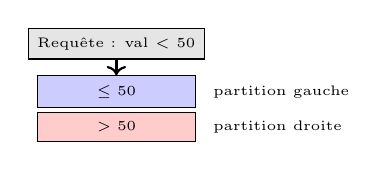
\begin{tikzpicture}[
                node distance=0.4cm,
                block/.style={draw, fill=blue!15, minimum width=2cm,
                              minimum height=0.35cm, font=\tiny}
            ]
            \node[block, fill=gray!20] (q1) {Requête : val $<$ 50};
            \node[block, below=0.2cm of q1, fill=blue!20] (l)  {$\leq 50$};
            \node[block, below=0.05cm of l,  fill=red!20]  (r)  {$> 50$};
            \draw[->, thick] (q1) -- (l);
            \node[right=0.1cm of l, font=\tiny] {partition gauche};
            \node[right=0.1cm of r, font=\tiny] {partition droite};
            \end{tikzpicture}
        \end{block}
        \vspace{0.15cm}
        \begin{alertblock}{Compromis}
            \footnotesize
            Performances optimales atteintes après plusieurs requêtes (« warm-up »).
        \end{alertblock}
    \end{columns}
\end{frame}

% =================================================
\section{Conclusion}
% =================================================

\subsection{Conclusion}

\begin{frame}{Résumé}
    \vspace{0.3cm}
    \begin{beamercolorbox}[
        wd=\textwidth, rounded=true, shadow=true,
        sep=8pt, center
    ]{title}
        {\Large\bfseries Conclusion}
    \end{beamercolorbox}
    \vspace{0.4cm}
    \begin{itemize}
        \item Les bases des Systèmes de Gestion de Base de Données
        \item Différentes optimisations utilisant l'algèbre relationnelle
        \item Optimisations dépendantes des données (indexation, cracking, stockage colonne)
        \item Une analyse comparative des résultats obtenus
    \end{itemize}
\end{frame}

\subsection{Nos ressources}

\begin{frame}{Nos ressources}
    \textbf{Bibliographie :}
    \begin{itemize}
        \item \href{https://drive.google.com/file/d/1KNmuRBf8CV-s-zqdkUEP8iyYlPgFiglb/view?usp=drive_link}%
              {\textit{The Design and Implementation of Modern Column-Oriented Database Systems} (2013)}
        \item \href{https://web.stanford.edu/class/cs345d-01/rl/cstore.pdf}%
              {\textit{C-Store: A Column-oriented DBMS} (2005)}
        \item \href{https://link.springer.com/content/pdf/10.1007/s41019-020-00149-7.pdf}%
              {\textit{A Survey on Advancing the DBMS Query Optimizer} (2021)}
        \item \href{https://www.microsoft.com/en-us/research/wp-content/uploads/2024/12/Extensible-Query-Optimizers-in-Practice.pdf}%
              {\textit{Extensible Query Optimizers in Practice} (2024)}
        \item \href{http://webdam.inria.fr/Alice/}%
              {\textit{Foundation of Databases} (1995)}
    \end{itemize}
\end{frame}

\end{document}
